\chapter{Introduction}

Virtual Reality, Augmented Reality and Computer Generated Imagery are ubiquitous in our increasingly digitalized world. Whether for immersive games played on head-mounted displays, image filters on social media, or movie productions involving special effects (which includes most), mixing virtual and real objects and worlds is not only accepted, it is often even expected.

A key factor to making the combination of the real and the virtual believable to human perception is correct lighting. If a virtual object in a real scene is not lit correctly, this is immediately recognizable by a human viewer, and breaks immersion. In order to ensure sufficient visual quality, lighting has to be meticulously captured in scenes that will contain clearly visible virtual objects. This tends to be done by substituting the virtual object by one or several spheres with different reflective characteristics (e.g. mirrored surface). Since this capture needs to be done manually at every desired point, capturing the lighting conditions at different points of a scene is very time-consuming.

In order to research how this process of capturing illumination can be improved, a project started in 2019 at the Laboratoire de Vision et Syst\` emes Num\' eriques (Laboratory for Computer Vision and Computer Systems, LVSN) at the Universit\'e Laval in Qu\'ebec, Canada aims to make illumination capture faster and more intuitive. 
%The goal of this project is to make the process of capturing illumination faster and more intuitive.
As a result, instead of having to place a reflective sphere at every location where illumination data is required, the capturer is able to walk around in the scene, carrying a 360$^{\circ}$ camera that is recording images of the surroundings. From this captured data, the lighting at each point in the room is extrapolated.

This process can be broken down to three distinct steps:
\begin{enumerate}
\item Capture of data with a 360$^{\circ}$ camera
\item Synthesis of non-captured viewpoints so that illumination can be estimated at \emph{every} point of the scene
\item Generation of high-dynamic range (HDR) data from low-dynamic range image data which can be directly used as illumination input to light virtual objects
\end{enumerate}

The synthesis of non-captured 360$^{\circ}$ viewpoints in step 2 is the focus of this thesis. This step is necessary so that the capturer is not required to record the scene from each possible point but can just record parts of the scene. The missing points can then be synthesized later, which saves capture time and memory space.

In general, there are several different approaches to view synthesis, which take into account different amounts of information on the 3D geometry of the scene. On one end of the scale, as much geometry information as possible is extracted from the image. However, using 3D geometric information requires very high-quality 3D data, which is difficult to recover from images. Lower-quality data tends to lead to visually unappealing results. \todo{citation?} Newer 3D geometry approaches use neural rendering, including Karimi et al.'s *name of paper/thesis*, which is also a part of the project at the LVSN.

Next come approaches that use only some 3D geometry information, such as depth layers, usually known as 2.5D. Here, the image is split into x different layers, each with a distinct depth. The objects in the scene are then each associated with one of the layers.

Approaches at the other end of the scale use no geometry whatsoever. Since there is no distinct name for this, the term used in this thesis is \emph{pixel-based rendering}, since the synthesis is based solely on pixels, disregaring any semantic information. \todo{taxonomy graphic}
Pixel-based rendering works fairly well for regular, planar images but has seen little or no research as of yet for 360$^{\circ}$ images. To start filling this research gap, this thesis explores the possibilities of adapting pixel-based rendering for panoramic image data. \todo{ok, now it's really important to make a clean gap analysis}

%In general, there are two fundamentally different approaches to view synthesis: using 3D geometric information of the scene, or using only the captured image data without any geometry. Using 3D geometric information requires very high-quality 3D data, which is difficult to recover from images. Lower-quality data tends to lead to visually unappealing results \todo{citation?}. Newer 3D geometry approaches use neural rendering, including Karimi et al.'s *name of paper/thesis*, which is also a part of the project at the LVSN. Synthesizing viewpoints \emph{without} using geometry, which is known as image-based rendering, works fairly well for regular, planar images but has seen little or no research as of yet for 360$^{\circ}$ images. To start filling this research gap, this thesis explores the possibilities of adapting image-based rendering for panoramic image data. \todo{ok, now it's really important to make a clean gap analysis}

\todo{logically from the text flow, this should go after the problem statement, even though it is part of the motivation.} In addition to its applicability for the lighting estimation project at the LVSN, the synthesis of non-captured 360$^{\circ}$ viewpoints has relevance on its own: Panoramic imagery is often used in Virtual Reality, for example for viewing historic locations and building interiors, or as a backdrop for VR games. The ability to accurately synthesize uncaptured viewpoints could greatly improve these viewing experiences, for example by creating stereo images or improving sample density for smoother navigation.

Furthermore, the results of this thesis can be combined with approaches using 3D geometry in order to leverage the advantages of both.

%
%- in addition to its necessity to the lighting estimation project, synthesizing non-captured viewpoints has relevance on its own
%--> there is a lot of research into improving VR viewing experiences
%--> most of it is based on using 3D geometry of the scene

\section*{Problem Statement}


The two distinct approaches in view synthesis (i.e. using no 3D geometry at all versus using as much 3D geometry as possible) have previously been researched for different applications:
Pixel-based rendering has been explored for planar (regular) images, for example to create smoothly viewable stereo panoramas from casually captured video input by Richardt et al. \cite{megastereo}, and there have been approaches to synthesising panoramic viewpoints from 360$^{\circ}$ video input by estimating 3D geometry, for example from Huang et a. \cite{6dof}. However, there is little to no research on using pixel-based rendering for synthesizing views from 360$^{\circ}$ image input. \todo{maybe include a collection of papers grouped into 4 areas: panoramic input, planar input, 3d geometry, pixel-based rendering. Definitely put this in, but not here}

%As mentioned above, there are two different approaches to view interpolation: Image-based rendering, and approaches using 3D geometry. Image-based rendering has been explored for planar (regular) images, for example to create smoothly viewable stereo panoramas from casually captured video input by Richardt et al. \cite{megastereo}, and there have been approaches to synthesising panoramic viewpoints from 360$^{\circ}$ video input by estimating 3D geometry, for example from Huang et a. \cite{6dof}. However, there is little to no research on using image-based rendering for synthesizing views from 360$^{\circ}$ image input. \todo{maybe include a collection of papers grouped into 4 areas: panoramic input, planar input, 3d geometry, image-based rendering. Definitely put this in, but not here}

In order to examine the potential of this approach, this thesis evaluates how well 360$^{\circ}$ panoramic view interpolation works when using image-based rendering without any supplemental geometric information i.e. pixel-based rendering.

Quality is difficult to quantify in the context of human perception, so the evaluation is based on different factors: euclidean distance to the ground truth, and visual believability. In this case, visual believability is measured by way of a minimal user study. In order to be able to compare the quality difference of the extension from planar to panoramic images, planar image results are also subjected to the same evaluation.

\section*{Scope}
%
%The development of your systematic took work. Now, leverage it!
%- in the methodology: do you vary parameters over some of them? in which steps?
%--> refer to here
%- in the definition of scope: how does the other work (other student,
%  literature, products) fit into this space? Where does yours?


Many different variables come into play when capturing image data, such as the metadata stored by the camera, the type of scene, the physical distance between captures, and much more. For the LVSN project, these variables do not need to be examined exhaustively, so the scope of this thesis is limited accordingly:

\paragraph{Location and rotation information}
Casually captured input data can be very unpredictable, as the capturer may move and rotate the camera freely. The captures used in this evaluation contain locational and rotational information in order to eliminate preprocessing steps such as simultaneous localization and mapping (SLAM).

\paragraph{Degrees of freedom}
The camera captures in three-dimensional space, so the convex hull spanned by the captures is also three-dimensional. In this context, the convex hull describes the 3D volume that is spanned by all points where sample images have been recorded. Interpolation is explored in all three dimensions, starting with 1D interpolation on a line between two captures, then extending to 2D interpolation on a plane and then extending to the 3D convex hull. The differentiation between synthesizing images within the convex hull and outside of the convex hull is that ...
%TODO explain convex hull in my context and clarify its importance to the work

\paragraph{Physical distance between captures}
The application of the LVSN project is for indoor scenes only, so the captures are within standard interior settings. This means that the distances between single captures are between approximately 0.5~m and 3~m.

\paragraph{Dynamics of samples}
All of the captures are of static surroundings.

\paragraph{Variation of scene distance to the camera}
The objects in the interior scenes have mostly uniform distance to the camera. The effects of larger variations of distances are also looked into.

\paragraph{Test methods}
In order to compare the synthesized views with the ground truth, the ground truth is captured as well. For the 1D case this works as follows: Three captures (A, B, C) are recorded that are linearly spaced on a line. Then, B' is interpolated from A and C. Then B' is compared to B by using $[metric]$.
%- predictability of capture location (tripod, hand-held, rig)
%  --> start with tripod, goal is hand-held
%- physical distance between samples
%  --> captures are only within standard interior settings, so distance is between approx 0.5 and 3m
%- knowledge of geometry
%  --> no geometry used in this project
%- dynamics of samples (static surroundings, some moving objects, lots of movement)
%  --> static surroundings for this project
%- distance of surroundings to camera (near-far large or small --> motion parallax visible or not)
%  --> interior scenes with most objects at a uniform distance (extend as bonus)
%- evaluation (visual believability: user study/personal evaluation, measurable metric)
%  --> personal evaluation of visual believability and mathematical comparison to ground truth (using cielab color space and euclidean distance)

%- in the definition of scope: how does the other work (other student,
%  literature, products) fit into this space? Where does yours?
\todo{star diagram of the dimensions}

\section*{Methodology}

\textbf{
\begin{figure}[]
\centering
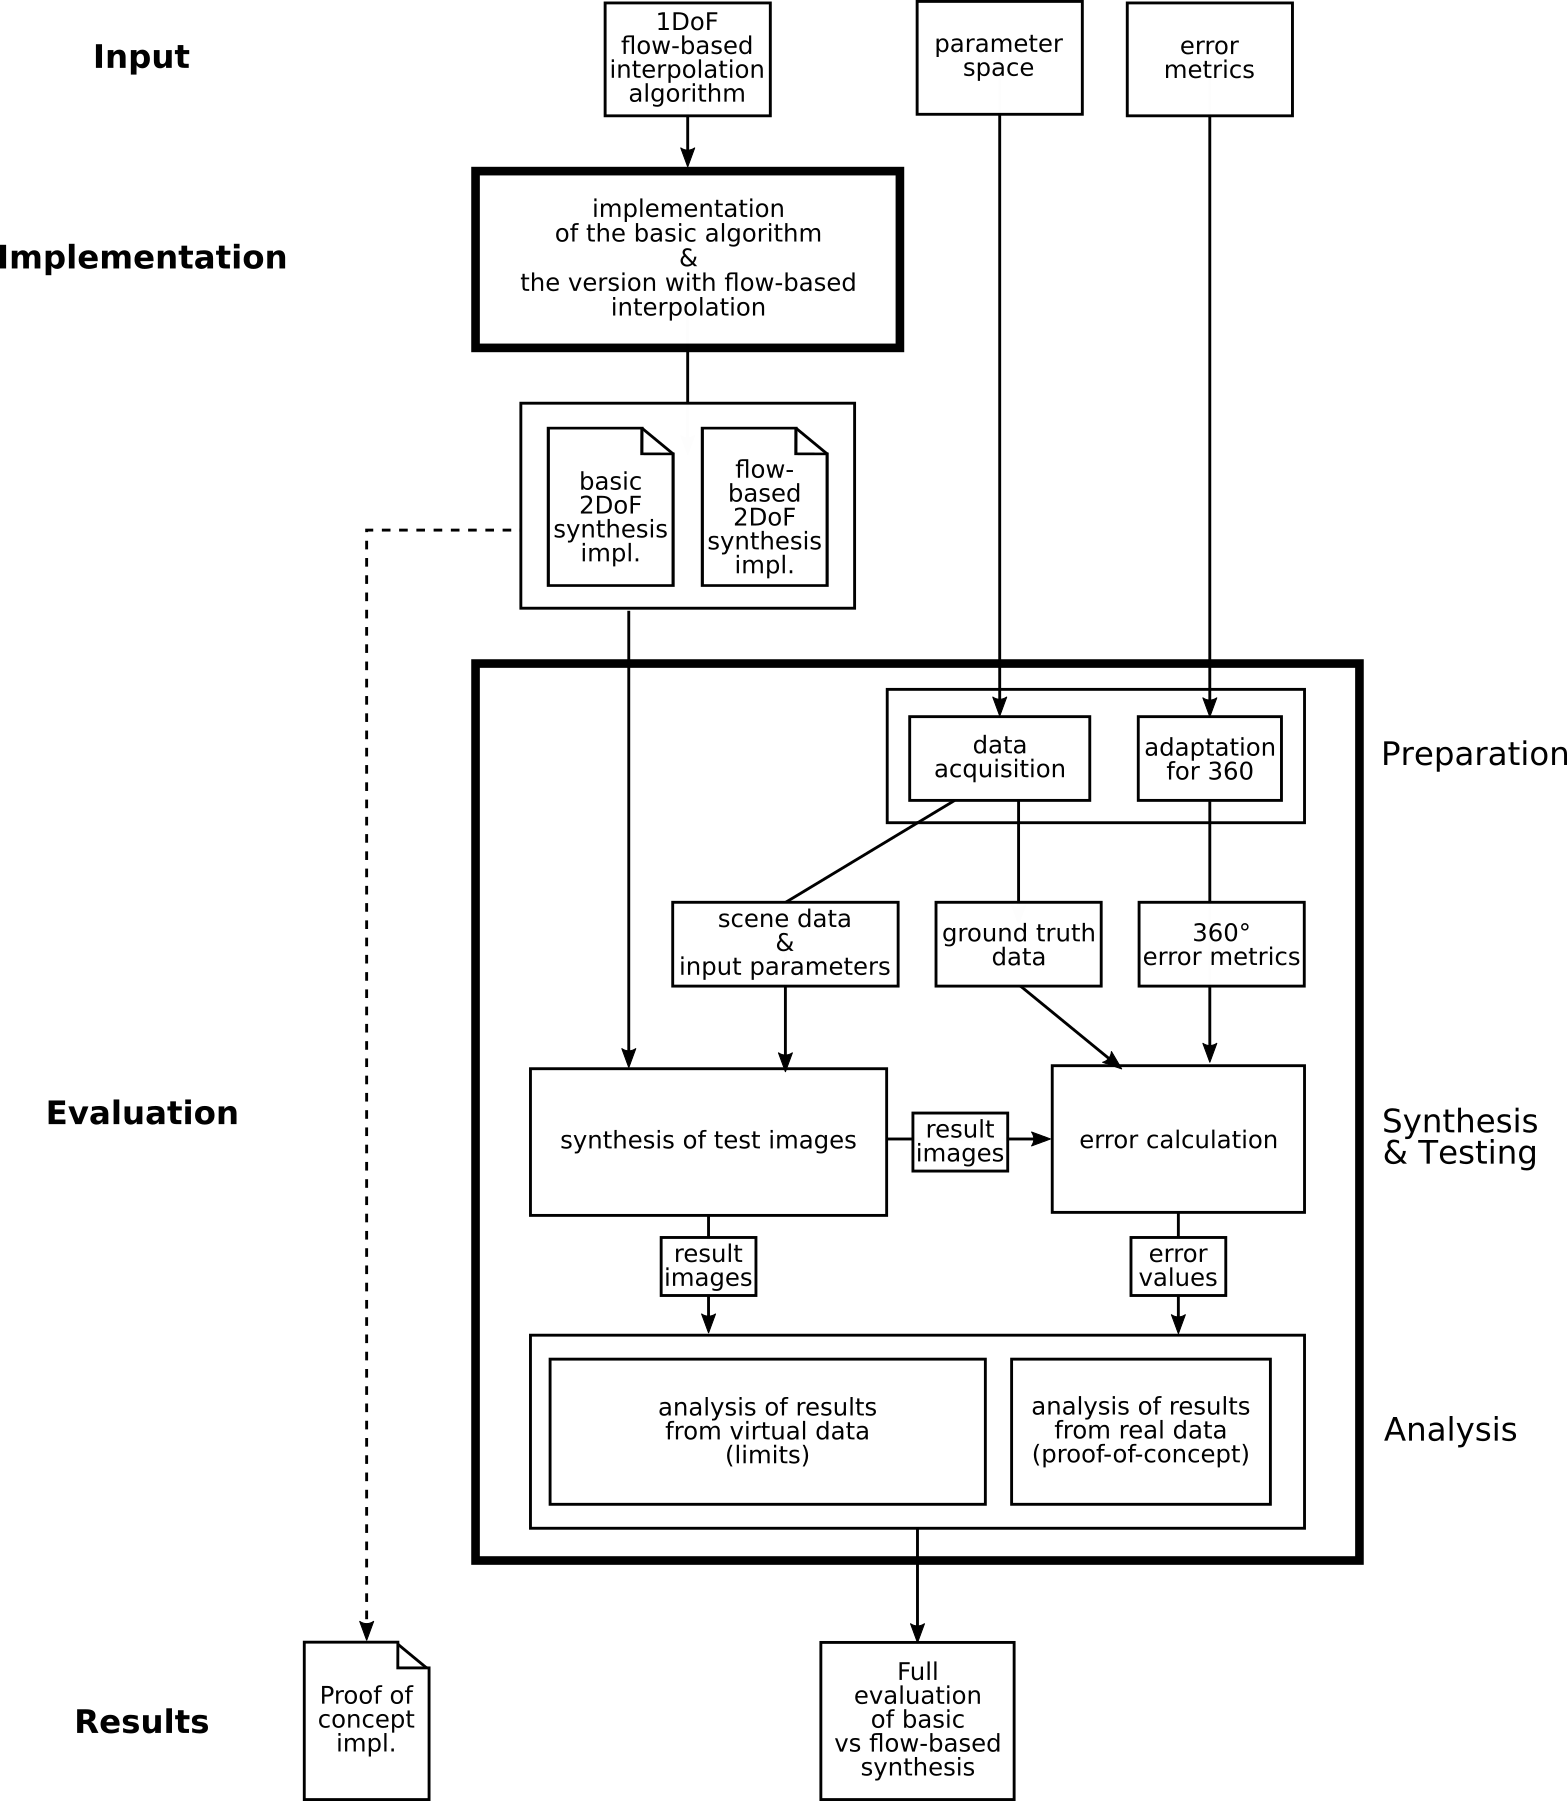
\includegraphics[width=1\textwidth]{methodology.png}
\caption{Methodology}
\label{fig:methodology}
\end{figure}
}

%art der testresultate
%
%structure and elements
In order to evaluate 360$^{\circ}$ panoramic view interpolation, this thesis follows a methodology with two distinct, alternating phases: experimentation and evaluation (Figure~\ref{fig:methodology}). Each experimentation step yields an implementation which produces synthesized 360$^{\circ}$ views that are then judged in the evaluation step. 
If the quality is deemed adequate, the next step of experimentation follows, which again will yield an extended implementation and test results. If the quality is not sufficient, the algorithm leading to the inadequate result is modified. This continues until the last experimentation step is successfully completed. 
%The implementations in the experimentation steps build on each other and each evaluation step is the same apart from minor details, since the test result images are always of the same type, i.e. a synthesized 360$^{\circ}$ image.

The base algorithm presented by Richardt et. al \cite{megastereo} is used as a starting point. This algorithm utilizes optical flow in its interpolation approach, which has to be adapted for 360 degrees as a preprocessing step. Along with the base algorithm, the input also consists of a set of test images that are used for testing after each experimentation step. These images are all 360$^{\circ}$ panoramas containing location and rotation information, taken at various points in 3D space in order to be able to test the different degrees of freedom. An appropriate subset is used for each experimentation step, exept for the last step, where all test images can potentially be used.
In the first experimentation step, view interpolation is implemented in 1D space, i.e. on a line between two sample images. The algorithm is then tested on a subset of sample images that are appropriate for . Assuming the results are acceptable, the 1D algorithm is used as a base to implement the 2D interpolation. The goal of the 2D interpolation is to be able to interpolate on a 2D plane spanned by several samples. This includes selecting appropriate views to then interpolate recursively using the 1D implementation. This is again tested on a subset of data and evaluated. In the last experimentation step, the 2D implementation is extended to three dimensions, so that any view within the convex hull of captures can be interpolated. This is then tested on all images and the results are again evaluated.
\todo{incorporate chapters:\\
1. introduction \\
2. state of the art \\
3. experimentation \\
3.1 1D implementation and evaluation \\
3.2 2D implementation and evaluation \\
3.3 3D implementation and evaluation \\
4. Final evaluation and results }

\section*{Results}

The results of this work are:
\begin{itemize}
\item an implementation of 360\degree view interpolation with 3DOF for scenes with no geometry
\item an implementation of 360\degree view interpolation with 2DOF using flow-based blending to alleviate artefacts caused by not using 3D geometry
\item an extensive evaluation that describes the quality of 360$^{\circ}$ panoramic view interpolation using image-based rendering without any supplemental geometric information
\item evaluation methodology for 360\degree images, including models and samples that can be used for benchmarking other methods
\end{itemize}

The results of this thesis can be the basis of various future work. For example, the range of application can be extended to outdoor scenes, or to scenes with higher variation in distances to the camera. In these cases, the result implementation can be used as a base and the the problems and limitations found in the evaluation can be utilized as guidelines. Furthermore, it could be valuable to explore the possibility of combining this image-based rendering approach with approaches that use 3D geometry.

